\section{Proposal}

\subsection{Motivation}

In the last half decade, advancements in Natural Language Processing (NLP) have been predominantly driven by Deep Learning (DL) models. One of the main advantages of DL models is their ability to function as efficient universal approximators; thereby approximating arbitrarily complex functions and logic programs \citep{cybenko1989approximation, hornik1989multilayer, kepner2018sparse}. Besides universal approximation capabilities, cross-validation heuristics help to identify DL models that are generalizable on unseen data sets. As a result, DL models offer decent approximation and generalization capabilities on arbitrary tasks given the appropriate model architecture and hyperparameter configurations.

In recent times and especially in NLP, DL models have been following trajectories of over-parameterization for better approximation and convergence on complex training tasks. Recent studies suggest that the practice of over-parameterization in non-convex optimization environments leads to a combinatorially large number of optimal solutions \citep{kepner2018sparse}. Given this and our previous perceptions, we postulate that current DL techniques offer the ability to produce \textit{multiple} generalizable models to complex tasks. 

\begin{gather}
  \label{eq:1}
  \overbrace{\text{Approximation} \oplus \text{Generalization}}^{\text{DL models + Cross-validation heuristics}} \Rightarrow \overbrace{\text{Semanticity}}^{\text{Human in the loop}}
\end{gather}

We argue that the next frontier for DL is the process of selecting semantically relevant models; or otherwise models that actually reflect meaningful considerations which humans could easily pick out and which are not dependent on spurious statistical artifacts. The most direct approach for this could be to involve the human in the loop; whereby the model exposes its internal mechanisms and the human evaluates its relevance and meaningfulness. This idea is reflected above in schematic \ref{eq:1}.

While seemingly straightforward, this process of semantic model selection is undermined by the generally unexplainable nature of DL models compared to classical machine learning models such as decision trees \citep{arrieta2020explainable}. This inherent lack of explainability in DL models further contributes to downstream issues such as adversarial vulnerabilities and ethical conflicts based on data biases \citep{doran2017does}. We therefore make an argument for extensive research into the explainability of DL models.

\subsection{Explainable artificial intelligence}

\citet{doran2017does} conduct a review of Explainable Artificial Intelligence (XAI) based on corpus-level analyses of NIPS, ACL, COGSCI and ICCV/ECCV papers. Based on their analysis, they characterize AI systems into three mutually exclusive categories of explainability; namely \textit{opaque systems} that offer no insight into internal model mechanisms, \textit{interpretable systems} where users can mathematically analyze internal model mechanisms and \textit{comprehensible systems} that emit symbols which enable explanations for how conclusions are reached. The study then culminates in the introduction of \textit{truly explainable systems}, where automated reasoning is central to the model's internal mechanisms without significant post-processing for explanation generation.

\citet{arrieta2020explainable} provide an extensive review of XAI techniques for a spectrum of machine-learning models. We deem this study as very useful because it provides both machine-learning users and practitioners a broad perspective of XAI methodologies. A key part of this study is its focus on post-hoc explainability techniques, which are explainability techniques reserved for models that are not readily interpretable by design. One useful subset of post-hoc explainability in DL would be explanation by simplification, which refers to the process of building a simpler and more explainable model (hereby referred to as a ``mimic'' model) which resembles the functionalities of its antecedent (hereby referred to as an ``oracle'' model). It is important to note that explanation by simplification focuses on building \textit{global} mimic models and not \textit{local} mimic models which resemble subsets of the oracle model, as is the case for the Local Interpretable Model-agnostic Explanations algorithm (LIME; \citealt{DBLP:journals/corr/RibeiroSG16}).

\subsection{Explanation by simplification}

Explanation by simplification is generally a difficult task because of natural trade-offs between the oracle model's performance and the mimic model's capacity for explainability \citep{arrieta2020explainable}. It is therefore vital to limit the loss in oracle model performance while maximizing the capacity for the mimic model's explainability. With this in light, we now look into two explanation by simplification techniques used in sequence learning and NLP.

\subsubsection{Simplification of arbitrary oracles}

\citet{hou2018learning} propose a simplification algorithm for producing mimic Finite State Automata (FSA) from arbitrary RNN oracle models. This is done by clustering the hidden states of RNNs based on token-level activations. Strongly clustered hidden states are then grouped together to represent states of a global FSA. A more complex algorithm for producing mimic Weighted Finite State Automata (WFSA) from arbitrary probabilistic oracle models is proposed by \citet{DBLP:journals/corr/abs-1905-08701}. While learning from arbitrary oracles is seen as advantageous in these studies, we argue that simplification of such arbitrary oracles could lead to mimic models that are not representative of the original oracles. This could negatively impact both the replication of oracle performance and the ability for mimic models to explain the internal mechanisms of their oracles.

\subsubsection{Simplification of constrained oracles}
\label{constrained}

To address the aforementioned limitations, we instead look into simplification techniques that use a constrained subset of oracles and mimics which have similar internal mechanisms. In some ways, this can be seen as a process of minimizing a hypothetical ``distance'' between oracles and mimics. \citet{schwartz2018sopa} propose a hybridized oracle RNN, CNN and WFSA neural architecture called \textbf{So}ft \textbf{Pa}tterns (SoPa). SoPa analyzes soft patterns in sequential data and enables simplification of the oracle model into an ensemble of WFSA mimics. \citet{wang2019state} propose novel oracle RNN architectures which include discrete centroids that enable smoother simplification into mimic FSA. Similarly, \citet{jiangcold} provide a novel oracle RNN architecture which allows for smoother simplification into regular expressions. 

\subsection{SoPa}

Based on literature review, source code analyses and email correspondence with all three authors of the studies listed in section \ref{constrained}; we deem further research into SoPa to be the most feasible given the timeline for this thesis. As SoPa is a complex hybrid neural architecture, we explain its mechanisms briefly and defer the reader to the article for a more in-depth understanding.

\begin{figure*}
  \centering 
  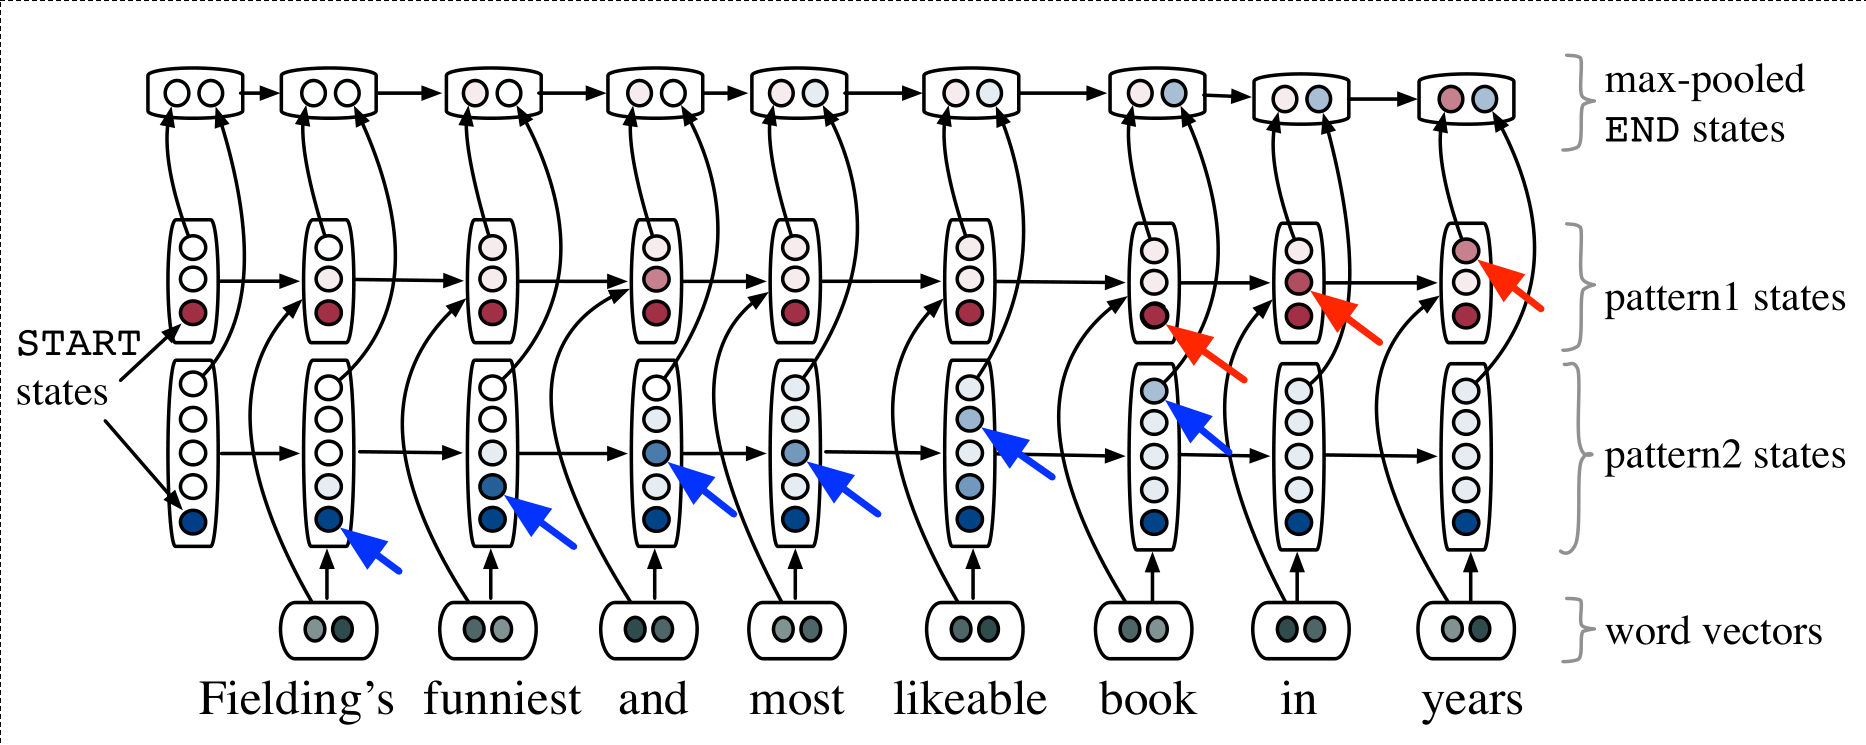
\includegraphics[trim={0.5cm 0cm 0cm 0.5cm},clip,width=\textwidth]{sopa.png} 
  \caption{Schematic of the SoPa neural architecture \citep{schwartz2018sopa}}
  \label{sopa}
\end{figure*}

\subsubsection{Overview}

As mentioned previously, SoPa is a hybridized RNN, CNN and WFSA neural architecture whose internal mechanisms are illustrated in Figure \ref{sopa}. SoPa resembles a RNN, CNN and WFSA in the following ways:

\paragraph{RNN:} SoPa is a recurrent model which processes tokens one after another. It has a simple recurrent activation function and no external memory.

\paragraph{CNN:} Important hyperparameters in SoPa are the number and length of patterns to learn. Since these patterns have a fixed window size, they resemble extensions of one-layer CNNs.

\paragraph{WFSA:} SoPa is designed to resemble a linear-chain WFSA with self-loops and limited $\epsilon$-transitions. These are realized by the construction of a transition matrix, much like the case for learning WFSA directly from input data.

\subsubsection{Performance}

\citet{schwartz2018sopa} tested the performance of SoPa on text classification tasks, specifically focusing on binary sentiment polarity detection. SoPa was shown to be competitive against BiLSTM and CNN baselines while using significantly fewer hyperparameters. SoPa was also shown to perform significantly better under small data settings. 

\subsubsection{Explanation by simplification}

The trained SoPa model consists of a transition matrix (or tensor) populated along its diagonals with token and position-specific transition weights. The transition matrix and input pattern hyperparameters can be simplified into textual patterns that fit them best using clustering algorithms. This could be used to identify word-level patterns that were important for the model's classification decisions. These patterns resemble regular expressions with $\epsilon$-transitions and wildcards. A sample pattern for positive sentiment is shown in Figure \ref{fsa}. \citet{schwartz2018sopa} utilize occlusion to determine which patterns contribute most to positive or negative sentiment.

\begin{figure*}
  \centering 
  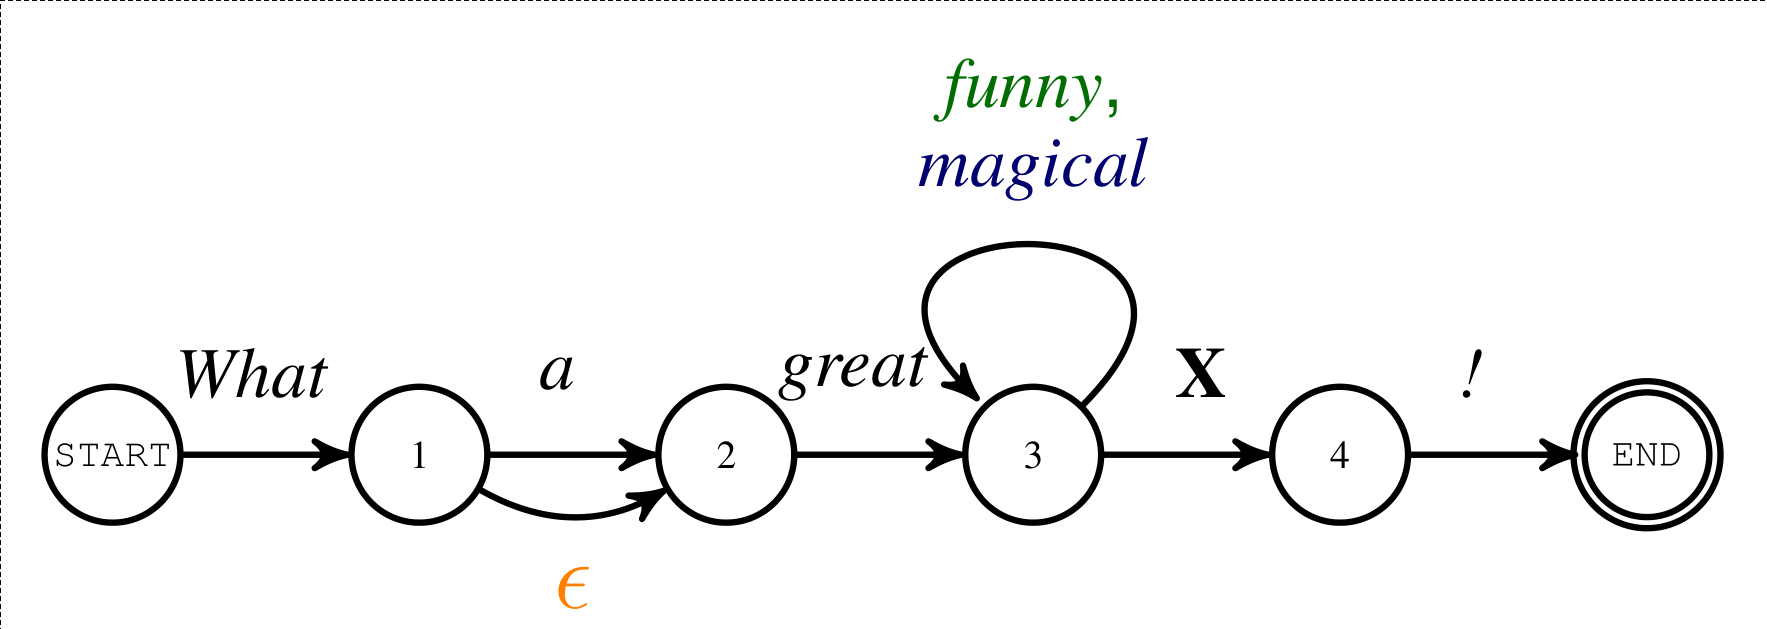
\includegraphics[trim={0.5cm 0cm 0cm 0.5cm},clip,width=0.7\textwidth]{fsa.png} 
  \caption{Example mimic FSA simplified from SoPa and its corresponding WFSAs \citep{schwartz2018sopa}}
  \label{fsa}
\end{figure*}

\subsubsection{Limitations}
\label{sopa-limitations}

There are several limitations to the current SoPa architecture which were verified through contact with the author(s):

\begin{enumerate}
  \item SoPa utilizes static word-level token embeddings which might contribute to less dynamic learning and more overfitting towards particular tokens.
  \item SoPa encourages minimal learning of wildcards/self-loops and $\epsilon$-transitions, which leads to increased overfitting on rare words such as proper nouns.
  \item While SoPa provides an interpretable architecture to learn discrete word-level patterns, it is also utilizes occlusion to determine the importance of various patterns. Occlusion is usually a technique reserved for uninterpretable model architectures and contributes little to global explainability.
  \item SoPa was only tested empirically on binary text classification tasks.  
\end{enumerate}

\subsection{SoPa++}

In response to the above limitations, we propose an extension to the SoPa architecture: SoPa++. The exact details of the extension might vary slightly based on time and resources. However a list of open tasks corresponding one-to-one with the limitations listed in section \ref{sopa-limitations} is provided below:

\begin{enumerate}
  \item Leverage dynamic sub-word-level embeddings from recent advancements in Transformer-based language modeling.
  \item Modify the architecture and hyperparameters to use more wildcards or self-loops, and verify the usefulness of these in the mimic WFSA models.
  \item Modify the output multi-layer perceptron layer to a general additive layer, such as a linear regression layer, with various basis functions. This would allow for easier interpretation of the importance of patterns without the use of occlusion.
  \item Test SoPa++ on multi-class text classification tasks, focusing particularly on Natural Language Understanding (NLU) tasks with existing benchmarks. One example is the RASA NLU benchmark \citep{bocklisch2017rasa} which contains numerous English language tasks for single-sequence multi-class intent classification. 
\end{enumerate}

\subsubsection{Research questions}

Based on the aforementioned tasks, we formulate three research questions:

\begin{enumerate}
  \item To what extent does SoPa++ contribute to competitive performance on NLU tasks?
  \item To what extent does SoPa++ contribute to improved explainability by simplification?
  \item What interesting and relevant explanations does SoPa++ provide on NLU task(s)?
\end{enumerate}

% LocalWords:  XAI ACL COGSCI ICCV ECCV interpretable connectionist NLP ANNs et
% LocalWords:  generalizable approximators NLU explainability al automata DL
% LocalWords:  hyperparameter parameterization combinatorially hoc FSA
% LocalWords:  Semanticity unexplainable RNN RNNs activations WFSA SoPa
% LocalWords:  centroids CNNs BiLSTM hyperparameters WFSAs embeddings
% LocalWords:  overfitting uninterpretable RASA SOTA perceptron

%%% Local Variables:
%%% mode: latex
%%% TeX-master: "main"
%%% End: